\documentclass{article}
\usepackage[utf8]{inputenc}
\usepackage[english]{babel}
\usepackage{amssymb}
\usepackage{amsmath}
\usepackage{graphicx}
\usepackage{enumerate}
\usepackage{longtable}
\usepackage{tikz}
\usetikzlibrary{automata, positioning}

\usepackage{geometry}
\geometry{left=2.5cm,right=2.5cm,top=2cm,bottom=2cm}

\setlength{\parskip}{0.5em}
\setlength{\parindent}{0em}
\renewcommand{\baselinestretch}{1.0}

\title{Assignment 2}
\author{COL 352\\
    Introduction to Automata \& 
    Theory of Computation}
\date{}

\begin{document}
    \maketitle
    
    \section*{Problem 1} Design DFA for the following languages over $\{0, 1\}$
    \begin{enumerate}[(a)]
        \item The set of all strings such that every block of of five consecutive symbols have at least two 0’s
        \item The set of strings with an equal number of 0’s and 1’s such that each prefix has at most one more 0 than
1’s and at most one more 1 than 0’s
    \end{enumerate}
    
    \textbf{Solution} : 
    
    (a) The DFA can be specified as a 5-tuple $<Q, \Sigma, s, F, \delta>$. The set of all states $Q$ is
    \begin{equation}
    \begin{aligned}
    Q~  = ~&\{\  s,~  q_{0},~  q_{1},~  q_{00},~  q_{01},~  q_{10},~
      q_{11},~  q_{000},~  q_{001},~  q_{010},~  q_{011},~  q_{100},~  q_{101},~  q_{110},~  q_{111},~  q_{0000},~ \\
      & q_{0001},~  q_{0010},~  q_{0011},~  q_{0100},~  q_{0101},~q_{0110},~  q_{0111},~  q_{1000},~  q_{1001},~  q_{1010},~  q_{1011},~  q_{1100},~  q_{1101},~ \\
      &  q_{1110},~  q_{1111},~  q_{00000},~  q_{00001},~  q_{00010},~  q_{00011},~q_{00100},~  q_{00101},~  q_{00110},~  q_{00111},~  q_{01000},~  q_{01001},~ \\
      & q_{01010},~  q_{01011},~   q_{01100},~  q_{01101},~  q_{01110},~  q_{01111},~  q_{10000},~  q_{10001},~q_{10010},~  q_{10011},~  q_{10100},~  q_{10101},~\\
      &  q_{10110},~  q_{10111},~  q_{11000},~  q_{11001},~ q_{11010},~  q_{11011},~  q_{11100},~  q_{11101},~  q_{11110},~q_{11111}\ \} \nonumber
    \end{aligned}
    \end{equation}
    
    \quad The start state is $s$. Assuming that all the strings of length less than 5 are accepted, the set of final states
    \begin{equation}
    \begin{aligned}
    F~  = ~&\{\  s,~  q_{0},~  q_{1},~  q_{00},~  q_{01},~  q_{10},~
      q_{11},~  q_{000},~  q_{001},~  q_{010},~  q_{011},~  q_{100},~  q_{101},~  q_{110},~  q_{111},~  q_{0000},~ \\
      & q_{0001},~  q_{0010},~  q_{0011},~  q_{0100},~  q_{0101},~q_{0110},~  q_{0111},~  q_{1000},~  q_{1001},~  q_{1010},~  q_{1011},~  q_{1100},~  q_{1101},~ \\
      &  q_{1110},~  q_{1111},~  q_{00000},~  q_{00001},~  q_{00010},~  q_{00011},~q_{00100},~  q_{00101},~  q_{00110},~  q_{00111},~  q_{01000},~  q_{01001},~ \\
      & q_{01010},~  q_{01011},~   q_{01100},~  q_{01101},~  q_{01110},~  q_{10000},~  q_{10001},~q_{10010},~  q_{10011},~  q_{10100},~  q_{10101},~\\
      &  q_{10110},~  q_{11000},~  q_{11001},~ q_{11010},~  q_{11100}\ \} \nonumber
    \end{aligned}
    \end{equation}
    
    \quad The transition function $\delta$ is given in following table\\
    \begin{longtable}{|c|c|c|}
      \hline
      % after \\: \hline or \cline{col1-col2} \cline{col3-col4} ...
       \textbf{Current state} & \textbf{Next state at input 0} & \textbf{Next state at input 1} \\ \hline
      $s$ & $q_{0}$ & $q_{1}$ \\ \hline
      $q_{0}$ & $q_{00}$ & $q_{01}$ \\ \hline
      $q_{1}$ & $q_{10}$ & $q_{11}$ \\ \hline
      $q_{00}$ & $q_{000}$ & $q_{001}$ \\ \hline
      $q_{01}$ & $q_{010}$ & $q_{011}$ \\ \hline
      $q_{10}$ & $q_{100}$ & $q_{101}$ \\ \hline
      $q_{11}$ & $q_{110}$ & $q_{111}$ \\ \hline
      $q_{000}$ & $q_{0000}$ & $q_{0001}$ \\ \hline
      $q_{001}$ & $q_{0010}$ & $q_{0011}$ \\ \hline
      $q_{010}$ & $q_{0100}$ & $q_{0101}$ \\ \hline
      $q_{011}$ & $q_{0110}$ & $q_{0111}$ \\ \hline
      $q_{100}$ & $q_{1000}$ & $q_{1001}$ \\ \hline
      $q_{101}$ & $q_{1010}$ & $q_{1011}$ \\ \hline
      $q_{110}$ & $q_{1100}$ & $q_{1101}$ \\ \hline
      $q_{111}$ & $q_{1110}$ & $q_{1111}$ \\ \hline
      $q_{0000}$ & $q_{00000}$ & $q_{00001}$ \\ \hline
      $q_{0001}$ & $q_{00010}$ & $q_{00011}$ \\ \hline
      $q_{0010}$ & $q_{00100}$ & $q_{00101}$ \\ \hline
      $q_{0011}$ & $q_{00110}$ & $q_{00111}$ \\ \hline
      $q_{0100}$ & $q_{01000}$ & $q_{01001}$ \\ \hline
      $q_{0101}$ & $q_{01010}$ & $q_{01011}$ \\ \hline
      $q_{0110}$ & $q_{01100}$ & $q_{01101}$ \\ \hline
      $q_{0111}$ & $q_{01110}$ & $q_{01111}$ \\ \hline
      $q_{1000}$ & $q_{10000}$ & $q_{10001}$ \\ \hline
      $q_{1001}$ & $q_{10010}$ & $q_{10011}$ \\ \hline
      $q_{1010}$ & $q_{10100}$ & $q_{10101}$ \\ \hline
      $q_{1011}$ & $q_{10110}$ & $q_{10111}$ \\ \hline
      $q_{1100}$ & $q_{11000}$ & $q_{11001}$ \\ \hline
      $q_{1101}$ & $q_{11010}$ & $q_{11011}$ \\ \hline
      $q_{1110}$ & $q_{11100}$ & $q_{11101}$ \\ \hline
      $q_{1111}$ & $q_{11110}$ & $q_{11111}$ \\ \hline
      $q_{00000}$ & $q_{00000}$ & $q_{00001}$ \\ \hline
      $q_{00001}$ & $q_{00010}$ & $q_{00011}$ \\ \hline
      $q_{00010}$ & $q_{00100}$ & $q_{00101}$ \\ \hline
      $q_{00011}$ & $q_{00110}$ & $q_{00111}$ \\ \hline
      $q_{00100}$ & $q_{01000}$ & $q_{01001}$ \\ \hline
      $q_{00101}$ & $q_{01010}$ & $q_{01011}$ \\ \hline
      $q_{00110}$ & $q_{01100}$ & $q_{01101}$ \\ \hline
      $q_{00111}$ & $q_{01110}$ & $q_{01111}$ \\ \hline
      $q_{01000}$ & $q_{10000}$ & $q_{10001}$ \\ \hline
      $q_{01001}$ & $q_{10010}$ & $q_{10011}$ \\ \hline
      $q_{01010}$ & $q_{10100}$ & $q_{10101}$ \\ \hline
      $q_{01011}$ & $q_{10110}$ & $q_{10111}$ \\ \hline
      $q_{01100}$ & $q_{11000}$ & $q_{11001}$ \\ \hline
      $q_{01101}$ & $q_{11010}$ & $q_{11011}$ \\ \hline
      $q_{01110}$ & $q_{11100}$ & $q_{11101}$ \\ \hline
      $q_{01111}$ & $q_{11110}$ & $q_{11111}$ \\ \hline
      $q_{10000}$ & $q_{00000}$ & $q_{00001}$ \\ \hline
      $q_{10001}$ & $q_{00010}$ & $q_{00011}$ \\ \hline
      $q_{10010}$ & $q_{00100}$ & $q_{00101}$ \\ \hline
      $q_{10011}$ & $q_{00110}$ & $q_{00111}$ \\ \hline
      $q_{10100}$ & $q_{01000}$ & $q_{01001}$ \\ \hline
      $q_{10101}$ & $q_{01010}$ & $q_{01011}$ \\ \hline
      $q_{10110}$ & $q_{01100}$ & $q_{01101}$ \\ \hline
      $q_{10111}$ & $q_{01110}$ & $q_{01111}$ \\ \hline
      $q_{11000}$ & $q_{10000}$ & $q_{10001}$ \\ \hline
      $q_{11001}$ & $q_{10010}$ & $q_{10011}$ \\ \hline
      $q_{11010}$ & $q_{10100}$ & $q_{10101}$ \\ \hline
      $q_{11011}$ & $q_{10110}$ & $q_{10111}$ \\ \hline
      $q_{11100}$ & $q_{11000}$ & $q_{11001}$ \\ \hline
      $q_{11101}$ & $q_{11010}$ & $q_{11011}$ \\ \hline
      $q_{11110}$ & $q_{11100}$ & $q_{11101}$ \\ \hline
      $q_{11111}$ & $q_{11110}$ & $q_{11111}$ \\ \hline
    \end{longtable}
    
    \newpage
    
    (b) If there is no explanation of the states/DFA, at most 5/10 will be given.
    \begin{center}
        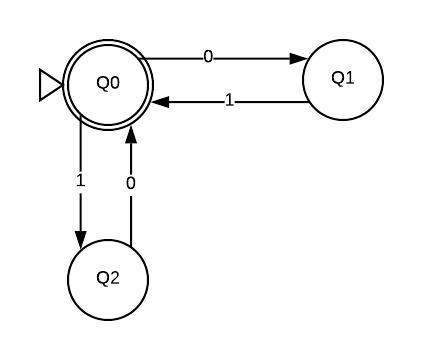
\includegraphics[width=0.5\textwidth]{Images/a2-q1-2.jpeg}
    \end{center}
    
    \section*{Problem 2} Design NFA for the following languages
    \begin{enumerate}[(a)]
        \item The set of strings over ${a, b}$ that have the same value when multiplied from left to right as from left to right. The rules of multiplication are $a \times a = b$, $b \times b = a$, $a \times b = b$, $b \times a = b$. Note that $((a \times b) \times b) = a$ and $(a \times (b \times b)) = b$, i.e. it is not associative
        \item The set of strings of the form $\{xwx^R ~|~ x, w$ are strings over 0,1 of non-zero length\}
    \end{enumerate}
    
    \textbf{Solution} : 

    (a) The problem reduces to finding strings of length at least 3 having the same initial and final characters. 
    
    \quad The NFA can be specified as a 5-tuple $<Q, \Sigma, s, F, \delta>$, with $Q = \{q_0,q_1,q_2,q_3,q_4,q_5,q_6,q_7,q_8\}$, $\Sigma = \{0,1\}$, 
    
    \quad Start state $s = q_0$ and accepting states $F = \{q_5 , q_6\}$

    \begin{center}
        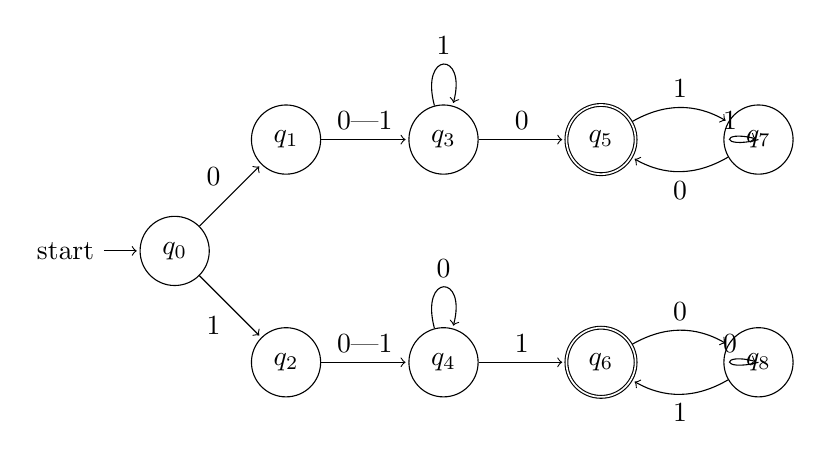
\begin{tikzpicture}[shorten >=1pt,node distance=2cm, on grid, auto] 
           \node[state,initial] (q_0)   {$q_0$}; 
           \node[state] (q_1) [above right=of q_0] {$q_1$}; 
           \node[state] (q_2) [below right=of q_0] {$q_2$};
           \node[state] (q_3) [right=of q_1] {$q_3$};
           \node[state] (q_4) [right=of q_2] {$q_4$};
           \node[state,accepting] (q_5) [right=of q_3] {$q_5$};
           \node[state,accepting] (q_6) [right=of q_4] {$q_6$};
           \node[state] (q_7) [right=of q_5] {$q_7$};
           \node[state] (q_8) [right=of q_6] {$q_8$};
            \path[->] 
            (q_0) edge  node {0} (q_1)
                  edge  node [swap] {1} (q_2)
            (q_1) edge  node  {0|1} (q_3)
            (q_3) edge  node  {0} (q_5)
                edge [loop above] node {1} ()
            (q_2) edge  node  {0|1} (q_4)
            (q_4) edge  node  {1} (q_6)
                edge [loop above] node {0} ()
            (q_5) [bend left] edge node  {1} (q_7)
            (q_6) edge  node  {0} (q_8)
        
            (q_7) edge  node  {0} (q_5)
                edge [loop above] node {1} ()
            (q_8) edge  node  {1} (q_6)
                edge [loop above] node {0} ();
        \end{tikzpicture}
    \end{center}
    
    (b) The following observations capture all possible strings with the following DFA
    
    \begin{enumerate}
        \item The product is '$a$' iff both the inputs are '$b$'
        \item The parity of the number of $b$'s to the leftmost $a$'s must be equal to number of $b$'s to the rightmost '$a$' iff both are non-empty. Let either of them be denoted by $L[a]$ and $L[a']$ respectively
        \item If  $L[a] = 0$  or $L[a'] = 0$, then parity of number of '$b$'s should be odd on the other side
        \item If $L[a] = 0$ and $L[a'] = 0$, then string is palindromic and gives the same result
    \end{enumerate}
    
    \begin{center}
        \begin{tikzpicture}[shorten >=1pt,node distance=2cm,on grid,auto] 
           \node[state,initial] (q_0)   {$q_0$}; 
           \node[state,accepting] (q_1) [above right=of q_0] {$q_1$}; 
           \node[state,accepting] (q_2) [below right=of q_0] {$q_2$};
           \node[state,accepting] (q_3) [right=of q_1] {$q_3$};
           \node[state,accepting] (q_4) [right=4cm of q_2] {$q_4$};
           \node[state] (q_5) [right=of q_3] {$q_5$};
           \node[state] (q_7) [above right=3cm of q_4] {$q_7$};
           \node[state,accepting] (q_8) [below right=3cm of q_4] {$q_8$};
           \node[state,accepting] (q_a) [below=7cm of q_2] {$q_a$};
           \node[state] (q_b) [right=4cm of q_a] {$q_b$};
           \node[state,accepting] (q_c) [above right=4cm of q_b] {$q_c$};
           \node[state] (q_d) [below right=4cm of q_c] {$q_d$};
            \path[->] 
            (q_0) edge node {a} (q_1)
                  edge node [swap] {b} (q_2)
            (q_1) edge node {a|b} (q_3)
            (q_3) edge node {b} (q_5)
                  edge [loop above] node {a} ()
            (q_2) edge node {a} (q_4)
                  [bend left] edge  node  {b} (q_a)
            (q_4) edge node {a} (q_7)
                  edge node {b} (q_8) ()
            (q_5) edge node {a|b} (q_3)
            (q_7) edge node {b} (q_8)
                  edge [loop right] node {a} ()
            (q_8) edge node {a|b} (q_7)
            (q_a) edge node {b} (q_2)
                  edge node {a} (q_b) ()
            (q_b) [bend right] edge node {b} (q_d)  
                  [bend left] edge node {a} (q_c) ()
            (q_c) edge node {b} (q_d)
                  edge [loop right] node {a} ()
            (q_d) edge node {a-b} (q_c);
        \end{tikzpicture}
    \end{center}

    
    \section*{Problem 3} Prove or disprove $(r+s)^* = r^* + s^*$, where $r$, $s$ and $t$ are regular expressions and $r=s$ implies $L(r)=L(s)$)
    
    \textbf{Solution} : Let $\Sigma = \{0, 1 \}$ and $r = 0^*$, $s = 1^*$
    
    Then, $(r + s)^* = \epsilon \cup \{ 0, 1 \} \cup \{ 0, 1 \}^2 \cup \dots$
    
    and, $r^* + s^* = \epsilon \cup \{ 0\} \cup \{ 0 \}^2 \cup \dots \cup \{ 1\} \cup \{ 1 \}^2 \cup \dots$
    
    Now, consider a string $01$.
    
    Clearly, $01 \in \{0, 1 \}^2 \Rightarrow 01 \in (r + s)^*$, but $01 \notin r^* + s^*$
 
    Hence, $(r+s)^* \neq  r^* + s^*$
    
    
    \section*{Problem 4} Which of the following are regular sets
    \begin{enumerate}[(a)]
        \item $\{ 0^{2^n} |~ n \geq 1\}$
        \item $\{ xx^Rw |~ x, w \in (0 + 1)^+ \}$
    \end{enumerate}
    
    \textbf{Solution} : 

    (a) Let $L$ denote the set, then assuming that it is regular, let $n \geq 1$ denote the pumping lemma constant

    \quad Consider the string $0^{2^n} \in L = 0^{p}0^{q}0^{r}$ with $p + q + r \geq n$, $q \geq 1$ and $p + q \leq n$. 
    
    \quad Now, from pumping lemma, $\forall i \geq 0,0 ^{p}0^{iq}0^{r} \in L$, i.e. $p + iq + r = 2^m$, for some $m \geq 1$. 
    
    \quad Setting $i = 2$, gives $p + 2q + r = 2^m$, and since $p + q + r = 2^n \Rightarrow 2^n + q = 2^m$, i.e. $q$ is a power of 2. 
    
    \quad Specifically, since $n, m$ are integers and $q \geq 1, q = 2^n$.
    
    \quad But this means that $q > n$, since $n \geq 1$
    and so, $p + q > n$  - a contradiction. Thus the $L$ is not a regular set.\\
    
    (b) Let $L$ denote the set, then assuming that it is regular, let $n \geq 1$ denote the pumping lemma constant
    
    \quad Consider the string $0^n1.10^n.1 \in L = 0^{l}0^{m}0^{n - m - l}1.10^n.1, ~1 \leq m < n, ~0 < l < n$, with $x = 0^l, ~ y = 0^{m}$
    
    \quad Now, from pumping lemma, $\forall i \geq 0, ~xy^iz \in L$, as $|xy| \leq n$ and $y \geq 1$

    \quad Setting $i = 2$, gives $xy^2z = 0^{n + m}1.10^n.1 \in L$ 
    
    \quad But since $n + m > n$, so $xy^2z \notin L$ - a contradiction. Thus the $L$ is not a regular set. \\

    \quad Also accepted : Solutions that use the Myhill-Nerode theorem correctly
    

    \section*{Problem 5} Is the set $\frac{1}{2}(L) = \{ x|~ \exists y$ such that $|x| = |y|, ~xy \in L \}$ regular?
    
    \textbf{Solution} : Since, $L$ is a regular language, so, let, $M = (Q,\Sigma, \delta, q_0, F)$ be the DFA that accepts $L$.
    
    Let $L' = \frac{1}{2}L $. We will construct a DFA $M' = (Q',\Sigma, \delta', q_0', F')$ which accepts $L'$ and hence prove that it is a regular language.
    \begin{itemize}
        \item $Q' = Q \times 2^Q $
        \item Let $S\in2^Q$. Define 
         $prev(S)= \{q \in Q\ | \ \exists\ a \in \Sigma,\ q' \in S\ s.t.\ \delta(q,a) = q'\}$
        \item $\delta'((q,S), a) = (\delta(q,a),prev(S))$
        \item $q_0' = (q_0,F)$
        \item $F' = \{(q,S), q\in S\}$
    \end{itemize}
    
    $F_1 = prev(F)$ will give us all the states in $M$ from where we can reach a final state of $M$ on reading a string of length 1. Similarly, $F_n = prev(F_{n-1})$ will give us all the states in $M$ from where we can reach a final state of $M$ on reading a string of length n.
    
    Let $xy \in L$ and $|x| = |y| = n$. $M$ reaches to a state $p$ after reading $x$ and from $p$ it reaches a final state $f$ on reading $y$. So, $p \in F_n$. And, on reading $x$, $M'$ will reach a state $(p, F_n)$. By definition of $F'$, it is a final state of $M'$. So, $xy$ will be accepted by $M'$.
    
    Now, let $x$ be accepted by $M'$ and $|x| = n$. So, let, $M'$ reaches a state $(p, P)$ where $p \in P$ on reading $x$. Also, $P = F_n$. So, there exists a string $y$, reading which we can reach from $p$ to a final state in $M$. So, $xy$ is accepted by $M$.

    Hence, $L'$ is the language accepted by $M'$.\\
    

    Regarding the grading:
    \begin{itemize}
        \item If you have simply specified the DFA with no explanation, you will get at most 5/10.
        \item You need to prove that any string in $\frac{L}{2}$ will be accepted by the DFA \textbf{AND} any string accepted by the DFA will be contained in $\frac{L}{2}$. 
    \end{itemize}
    
\end{document}
